% Apology to reader:

% The indentation in here is extremely weird, and you can see
% me struggle with trying to establish an indentation that I'm happy with. I
% once upon a time used to LaTeX with monstrous hundred or even thousand
% character lines, but I'm trying to move to a more code-like structure, and
% this document is a living testament to my struggles :(
    \documentclass[10pt]{article}
    \usepackage{fancyhdr, amsmath, amsthm, amssymb, mathtools, lastpage,
    hyperref, enumerate, graphicx, setspace, wasysym, upgreek, listings, times}
    \usepackage{geometry}
    \newcommand{\scinot}[2]{#1\times10^{#2}}
    \newcommand{\bra}[1]{\left<#1\right|}
    \newcommand{\ket}[1]{\left|#1\right>}
    \newcommand{\dotp}[2]{\left<#1\,\middle|\,#2\right>}
    \newcommand{\rd}[2]{\frac{\mathrm{d}#1}{\mathrm{d}#2}}
    \newcommand{\pd}[2]{\frac{\partial#1}{\partial#2}}
    \newcommand{\rtd}[2]{\frac{\mathrm{d}^2#1}{\mathrm{d}#2^2}}
    \newcommand{\ptd}[2]{\frac{\partial^2 #1}{\partial#2^2}}
    \newcommand{\norm}[1]{\left|\left|#1\right|\right|}
    \newcommand{\abs}[1]{\left|#1\right|}
    \newcommand{\pvec}[1]{\vec{#1}^{\,\prime}}
    \newcommand{\tensor}[1]{\overleftrightarrow{#1}}
    \let\Re\undefined
    \let\Im\undefined
    \newcommand{\ang}[0]{\text{\AA}}
    \newcommand{\mum}[0]{\upmu \mathrm{m}}
    \DeclareMathOperator{\Re}{Re}
    \DeclareMathOperator{\Im}{Im}
    \DeclareMathOperator{\Log}{Log}
    \DeclareMathOperator{\Arg}{Arg}
    \DeclareMathOperator{\Tr}{Tr}
    \DeclareMathOperator{\E}{E}
    \DeclareMathOperator{\Var}{Var}
    \DeclareMathOperator*{\argmin}{argmin}
    \DeclareMathOperator*{\argmax}{argmax}
    \DeclareMathOperator{\sgn}{sgn}
    \newcommand{\expvalue}[1]{\left<#1\right>}
    \usepackage[labelfont=bf, font=scriptsize]{caption}\usepackage{tikz}
    \usepackage[font=scriptsize]{subcaption}
    \everymath{\displaystyle}
    \lstset{basicstyle=\ttfamily\footnotesize,frame=single,numbers=left}

\tikzstyle{circ} = [draw, circle, fill=white, node distance=3cm, minimum
height=2em]

\begin{document}

\pagestyle{fancy}
\rhead{Yubo Su --- Tidbits}
\cfoot{\thepage/\pageref{LastPage}}

Welcome back to my random tidbits file! When I come up with interesting
problems, I will put them here.

\section{Probability Distributions and Weight Loss}

I was keeping track of my own weight when I realized that my scale was
sufficiently inconsistent that my weight loss was dominated by the statistical
noise. So then I was curious what the best way of mitigating this is, mean or
median of multiple measurements. One would suspect it's the mean, or one would
know simply by having taken any real statistics class, but I'm curious.

\subsection{Mean-based averaging}

This one is easy. Assume we have $n$ iid variables $X_i$ with mean $\mu$ and
variance $\sigma^2$, then the random variable corresponding to their average
$\expvalue{X_i}$ has mean $\mu$ and variance $\frac{\sigma^2}{n}$, so standard
deviation $\frac{\sigma}{\sqrt{n}}$. Thus, we have an unbiased estimator of the
true mean and a variance that falls off like $\sim n^{-1/2}$.


\subsection{Median-based averaging}

This one is a bit more fun. Let's start with $n=3$, then defining $f(x)$ the
probability density function and $F_X(x) = f_X(X \leq x)$ the cumulative
distribution function, the probability density of the median $f_\eta(y)$ is
given
\begin{align}
    f_\eta(y) = 6f_X(y)F_X(y)\left( 1 - F_X(y) \right)\label{1-eta}
\end{align}
the probability we choose one value greater than $y$ the median and one less,
multiplied by $6$ because there $3$ ways to choose which element is the median
and $\binom{2}{1}$ binomial coefficient for exactly one element on each side.
This seems to be a bit difficult to verify to be normalized in the general case,
or that
\begin{align}
    \int\limits_{-\infty}^{\infty}f_\eta(y)\;\mathrm{d}y &=
    \int\limits_{-\infty}^{\infty}\left[
        6f_X(y)\int\limits_{-\infty}^{y}f_X(\xi)\;\mathrm{d}\xi
        \int\limits_{y}^{\infty}f_X(\zeta)\;\mathrm{d}\zeta
    \right]\mathrm{d}y = 1
\end{align}

Let's just verify this in the uniform distribution case, and leave the general
oase as an exercise to brighter colleagues. We consider the normalized uniform
distribution $f_X(x) = 1, x \in [0,1]$, or $F_X(x) = x, x \in [0,1]$. We confirm
that the expression for $f_\eta$ is normalized:
\begin{align}
    \int\limits_{0}^{1}6y(1-y)\;\mathrm{d}y = 1
\end{align}

We then wish to examine whether $f_\eta(y)$ is an unbiased estimator of $\mu$.
Again, we begin with examining a sub-case, where $f_X(x)$ is symmetric about its
mean $\mu$. This yields that $F_X(\mu) = 0.5$ and is odd about
$\mu$\footnote{This is a slight abuse of terminology: we mean that $F_X(x - \mu)
- 0.5 = -(F_X(-(x-\mu)) - 0.5)$.} and so that $F_X(y)\left( 1 - F_X(y) \right)$
is also even/symmetric about $\mu$. Finally, this implies that $f_\eta(y)$ as
defined in \autoref{1-eta} is also symmetric about $\mu$ and we are done.

However, this analysis breaks down in the asymmetric case. We see that
$F_X(y)\left( 1 - F_X(y) \right)$ is \emph{always} symmetric about the
median $\eta$ of $f_X$, since $F_X(\eta) = 0.5$. In general, the mean and median
of a probability distribution are not equal, so there is no guarantee that
$\expvalue{f_\eta(y)} = \expvalue{f(y)}$, and indeed we can verify for some
contrived probability distribution such as
\begin{align}
    f_X(x) &=
    \begin{cases}
        2 & 0 \leq x \leq 0.25\\
        1 & 0.5 \leq x \leq 1\\
        0 & \text{else}
    \end{cases}
\end{align}
that $\expvalue{f_X(x)} = 0.4375$ while
\begin{align}
    \expvalue{f_\eta(y)} &= \int\limits_{0}^{0.25}24y^2(1-2y)\;\mathrm{d}y +
    \int\limits_{0.5}^{1}6y^2(1-y)\;\mathrm{d}y\\
    &\approx 0.4218
\end{align}

This should not have surprised us: we're trying to use a median to estimate the
mean of a distribution, and the two are equal when the PD is symmetric and
unequal otherwise.

The above analyses probably generalizes to median-of-$n$ trials, where with a
symmetric PD we have the being a unbiased estimator of the mean and with an
asymmetric an biased estimator, for any parity of $n$, but I'm too lazy to check
this out and will take it on faith. For reference, we assert the generalization
of \autoref{1-eta} below for odd $N = 2m+1$ trials below
\begin{align}
    f_{\eta, 2m+1}(y) &= N\binom{2m}{m} f_X(y)\left( F_X(y) \right)^m
        \left( 1 - F_X(y) \right)^m
\end{align}
which is simply generalizing to the concept of ``$m$ elements on either side of
$y$.''

It seems difficult to compare these median-based results (many of which could
probably be strengthened) to the mean based results in the case of an arbitrary
PDF, so let's specialize to a few tractable cases.

\subsection{Uniform Distribution}

I'm tired of not obtaining usable results, so let's simplify the discussion
considerably and assume that we have a uniform probability distribution, or that
$X \in [\mu - a, \mu + a]$. In this case the median-of-three also provides for
an unbiased estimator as shown above.  What is the variance of this estimator
then?

\subsubsection{Mean-based}

Let's first examine the results of a mean-based estimation of $\mu$. Call
$\hat{\mu}_N$ the estimator generated by averaging $N$ samplings, then we know
that $\expvalue{\hat{\mu}_N} = \mu$ by linearity of expectation and
$\sigma_{\hat{\mu}_N}^2 = \frac{\sigma_X^2}{N}$ by linearity of variance, so
it remains to compute $\sigma_X^2$, which is given by
\begin{align}
    \sigma_X^2 &= \expvalue{X^2} - \expvalue{X}^2\\
    &= \int\limits_{\mu - a}^{\mu + a}\frac{1}{2a}x^2\;\mathrm{d}x - \mu^2\\
    &= \frac{6\mu^2a + 2a^3}{6a} - \mu^2\\
    &= \frac{a^2}{3}
\end{align}

Thus, $\sigma_{\hat{\mu}_N}^2 = \frac{a^2}{3N}$.

\subsubsection{Median-based, $N=3$}

Now for the median-based approach. Denote $\tilde{\mu}_N$ the estimator
generated by taking the median of $N$ samplings, then we know that
$\expvalue{\tilde{\mu}_N} = \mu$ nonetheless because the uniform PD is a
symmetric probability distribution. It thus remains to compute
$\expvalue{\sigma^2_{\tilde{\mu}_N}}$. This seems nontrivial, so let's start
with $N=3$:
\begin{align}
    \expvalue{\tilde{\mu}_3^2} &= \int\limits_{-\infty}^{\infty}
        6f_X(x)F_X(x)\left( 1 - F_X(x) \right)\;x^2 \mathrm{d}x\\
        &= \int\limits_{\mu-a}^{\mu+a}
            \frac{6}{2a}\frac{x - (\mu - a)}{2a}\frac{(\mu + a) - x}{2a}x^2
            \;\mathrm{d}x\\
        &= \int\limits_{-a}^{a}\frac{6}{2a}\frac{a + y}{2a}\frac{a - y}{2a}
            (y + \mu)^2\;\mathrm{d}y\\
        &= \int\limits_{-a}^a\left[
                \frac{6}{8a^3}\left(
                    a^2y^2 + a^22y\mu + a^2\mu^2 - y^4 - 2\mu y^3 - y^2\mu^2
                \right)
            \right]\;\mathrm{d}y\\
        &= \frac{6}{8a^3}\left[
                \frac{(a^2 - \mu^2)y^3}{3} - \frac{y^5}{5}
            \right]_{-a}^a + \frac{3\mu^2}{2}\\
        &= \frac{6}{8a^3}\left[
            \frac{\left(
                a^2 - \mu^2
            \right) 2a^3}{3} - \frac{2a^5}{5}
        \right] + \frac{3\mu^2}{2}\\
        &= \mu^2 + \frac{a^2}{5}
\end{align}
and so $\sigma_{\tilde{\mu}_3}^2 = \frac{a^2}{5}$. Compare this to
$\sigma_{\hat{\mu}_3}^2 = \frac{a^2}{9}$ and we see that the mean-based
estimation has lower uncertainty.

\subsubsection{Median-based, arbitrary $N$}

Armed with this, let's also try to compute for arbitrary, odd $N=2m+1$, for which we
have
\begin{align}
    \expvalue{\tilde{\mu}_N^2}
        &=
            N\binom{2m}{m}\int\limits_{-a}^{a}\frac{1}{2a}
                \left( \frac{a^2 - y^2}{4a^2} \right)^m(y+\mu)^2
            \;\mathrm{d}y
\end{align}

Now, there's probably a cool combinatorial way to evaluate this, but let's just
care about asymptotic behavior. Then
\begin{align}
    \lim_{N \to \infty}\expvalue{\tilde{\mu}_N^2}
        &\approx
            N\frac{2^{2m}\sqrt{2m}}{m}\int\limits_{-a}^{a}
                \frac{1}{2a}\frac{1}{4^m}
                \left( 1 - \frac{y^2}{a^2} \right)^m (y+\mu)^2
            \;\mathrm{d}y\\
        &\approx \frac{1}{2a}\sqrt{8m}
            \int\limits_{-a}^{a}
                \left( 1 - \frac{y^2}{a^2} \right)^m(y+\mu)^2\;\mathrm{d}y
\end{align}
where we approximate $N \approx 2m$. Now, we know that $\left( 1-\frac{y^2}{a^2}
\right)^m$ is going to fall off sharply to $0$ as $y$ increases, so we can
approximate (for some normalization factor $A$)
\begin{align}
    \int\limits_{-a}^{a}\left( 1-\frac{y^2}{a^2} \right)^m\;\mathrm{d}y
        &\sim A
            \int\limits_{-a/\sqrt{m}}^{a/\sqrt{m}}
                1 - \frac{my^2}{a^2}
            \;\mathrm{d}y\label{1-two}\\
    \lim_{N \to \infty}\expvalue{\tilde{\mu}_N^2}
        &\approx \frac{A}{2a}\sqrt{8m}
            \int\limits_{-a/\sqrt{m}}^{a/\sqrt{m}}
                \left( 1 - \frac{my^2}{a^2} \right)(y+\mu)^2
            \;\mathrm{d}y
\end{align}
To compute $A$, we require that the coefficient of $\mu^2$ be $1$ so that the
difference $\expvalue{\tilde{\mu}_N^2} - \expvalue{\tilde{\mu}_N}^2$ does not
depend in first order on $\mu$. It's clear that since the integral is symmetric,
we need only consider even powers of $y$, and so our integral becomes
\begin{align}
    \lim_{N \to \infty}\expvalue{\tilde{\mu}_N^2}
        &= \frac{A\sqrt{8m}}{2a} \int\limits_{-a/\sqrt{m}}^{a/\sqrt{m}}
            \left( 1 - \frac{my^2}{a^2} \right)\left( y^2 + \mu^2 \right)
        \;\mathrm{d}y\\
        &= \frac{A\sqrt{8m}}{2a} \int\limits_{-a/\sqrt{m}}^{a/\sqrt{m}}
            \mu^2 + \left( 1 - \frac{m\mu^2}{a^2} \right)y^2 - \frac{my^4}{a^2}
        \;\mathrm{d}y\\
        &= \frac{A\sqrt{8m}}{2a} \left[
            \frac{2\mu^2a}{\sqrt{m}} + \left( 1 - \frac{m\mu^2}{a^2} \right)
                \left( \frac{2}{3}\frac{a^3}{m^{3/2}} \right) -
            \frac{2ma^5}{5a^3m^{5/2}}
        \right]\\
        &= A\frac{\sqrt{32}}{3}\mu^2 + A\frac{4\sqrt{2}}{15}\frac{a^2}{m}
\end{align}
and so we find that $A = \frac{3}{\sqrt{32}}$ and finally
\begin{align}
    \sigma_{\tilde{\mu}_N^2}^2 &= \frac{a^2}{5m}\label{1-result}
\end{align}

The agreement for $N=3, m=1$ is a bit uncanny, but let's try to verify this
computationally before jumping for joy.

This is a polynomial relationship on $m$, so we can sample $m$ logarithmically
to computationally verify our result. The obtained results are as follows in
\autoref{fig:1-medians}.
\begin{figure}[!h]
    \centering
    \begin{subfigure}{0.75\textwidth}
        \centering
        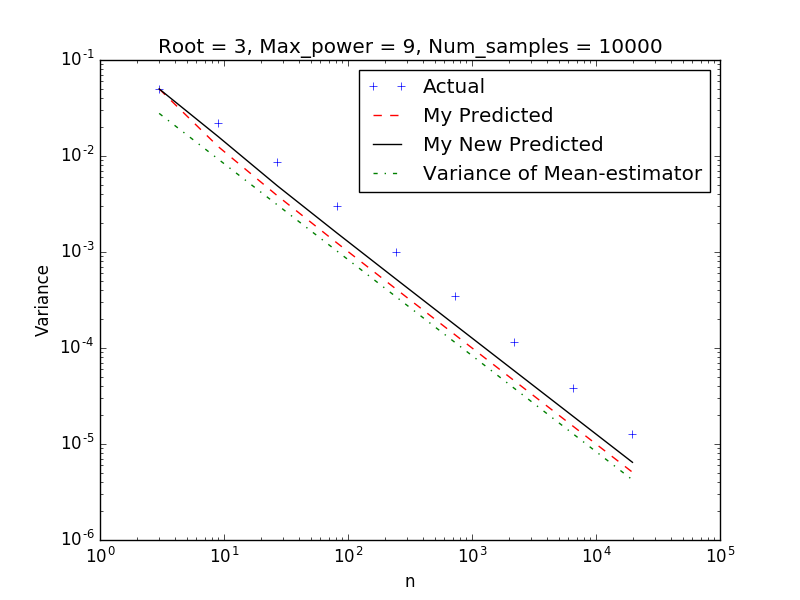
\includegraphics[width=\textwidth]{medians_asymptotic.png}
        \caption{Plot of medians as a function of $N$}
    \end{subfigure}
    \begin{subfigure}{0.75\textwidth}
        \centering
        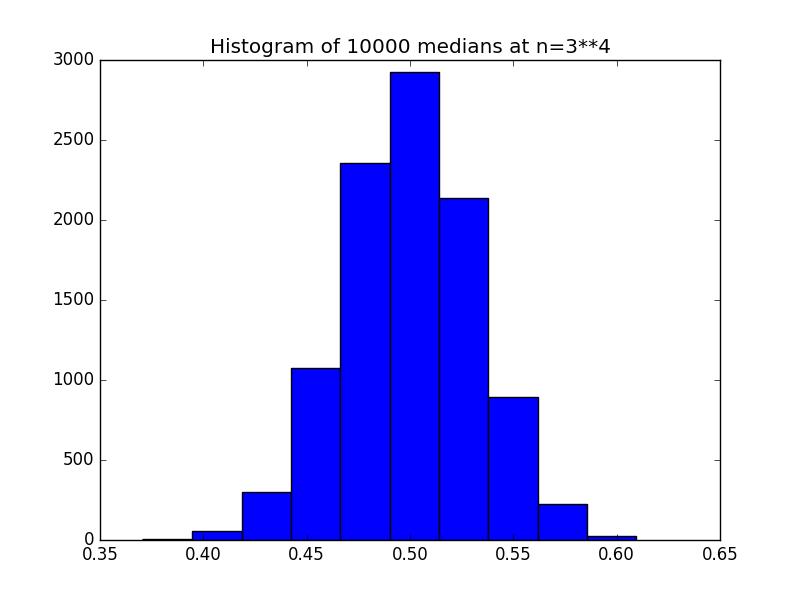
\includegraphics[width=\textwidth]{medians_slice_hist.png}
        \caption{Histogram of $1000$ medians at a single value of $N$}
    \end{subfigure}
    \caption{Computational results for our medians result. Used $\mu=0.5,
    a=0.5$, or a uniform sampling $[0,1]$. Sampled over $n=3^{[1, 9]}$ with
    $10000$ samples at each value of $n$.}
\label{fig:1-medians}
\end{figure}

The histogram is plotted merely out of curiosity, but seems to suggest a normal
distribution per the Law of Large Numbers. Nonetheless, \autoref{1-result}
seems to be slightly off. It perfectly agrees in the $N=3$ case as can be
verified by simulation, but eventually grows to be a factor of approximately $2$
off.

So it turns out our uncanny success for $N=3, m=1$ was a pure stroke of luck,
and our expression isn't precisely correct. Nonetheless, we can make a few plots
to figure out numerically how well median vs.\ mean based averaging performs,
and the degredation of our estimate over $N$. These plots are
\begin{figure}[!h]
    \centering
    \begin{subfigure}{0.45\textwidth}
        \centering
        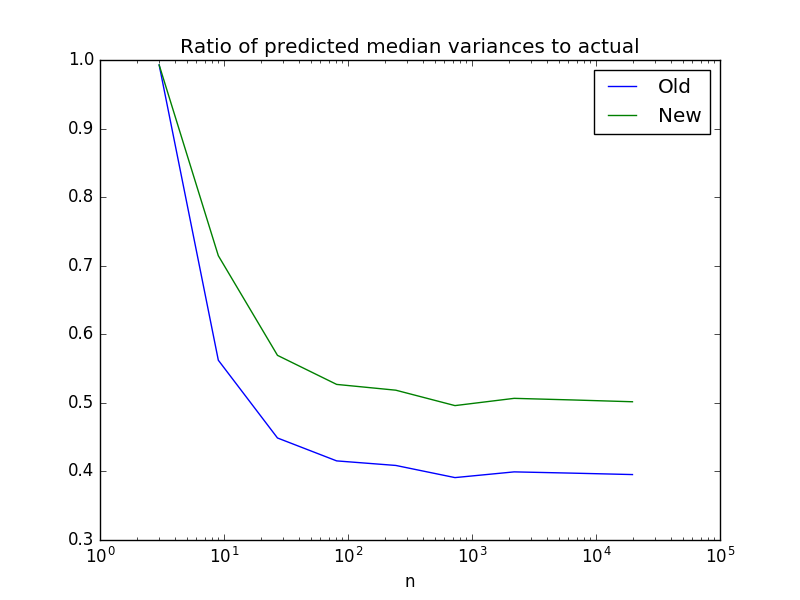
\includegraphics[width=\textwidth]{medians_ratio_to_real.png}
        \caption{Seems asymptotically close to $2/5, 1/2$ maybe?}
    \end{subfigure}
    \begin{subfigure}{0.45\textwidth}
        \centering
        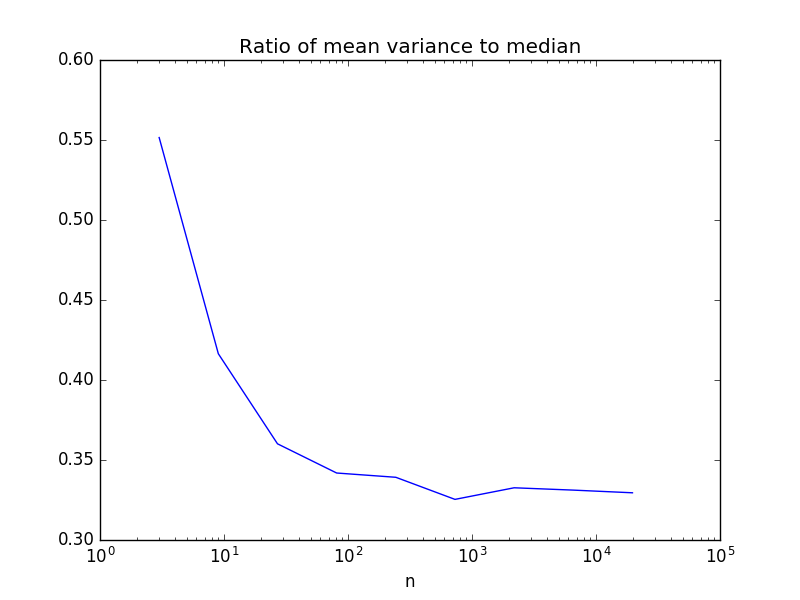
\includegraphics[width=\textwidth]{medians_ratio_to_mean.png}
        \caption{Seems asymptotically close to $1/3$?}
    \end{subfigure}
    \caption{A couple ratios of interest. Same sampling as in
    \autoref{fig:1-medians}.}
\label{fig:1-ratios}
\end{figure}

\subsubsection{Median-based, arbitrary $N$, reworked}

Let's try to include the truncated terms in $\left( 1 - \frac{y^2}{a^2}
\right)^m$, since they really are rather non-small compared to the leading term
that we kept. Where we had before put $1 - \frac{my^2}{a^2}$, we should instead
put
\begin{align}
    \left( 1 - \frac{y^2}{a^2} \right)^m
        &= \sum\limits_{k=0}^{m} \binom{m}{k}\left( -\frac{y^2}{a^2} \right)^k\\
    \lim_{N \to \infty}\expvalue{\tilde{\mu}_N^2}
        &\approx \frac{A}{2a}\sqrt{8m}
            \int\limits_{-a/\sqrt{m}}^{a/\sqrt{m}}
                \sum\limits_{k=0}^{m}\binom{m}{k}
                    \left( -\frac{y^2}{a^2} \right)^k
                (y+\mu)^2
            \;\mathrm{d}y
\end{align}

We approximate $\binom{m}{k} \approx \frac{m^k}{k!}$ since higher terms in $k$
are attenuated anyways. Using the same parity argument to kill the term odd in
$y$, we rewrite
\begin{align}
    \lim_{N \to \infty}\expvalue{\tilde{\mu}_N^2}
        &\approx \frac{A}{2a}\sqrt{8m}
            \int\limits_{-a/\sqrt{m}}^{a/\sqrt{m}}
                \sum\limits_{k=0}^{m}\frac{m^k}{k!}
                    \left( -\frac{y^2}{a^2} \right)^k
                (y^2+\mu^2)
            \;\mathrm{d}y
\end{align}

Examine first the $\mu^2$ coefficient
\begin{align}
    1
        &= \frac{A}{2a}\sqrt{8m}
            \sum\limits_{k=0}^{m}\frac{m^k}{k!}
                \int\limits_{-a/\sqrt{m}}^{a/\sqrt{m}}
                    \left( -\frac{y^2}{a^2} \right)^k
                \;\mathrm{d}y\\
        &= \frac{A}{2a}\sqrt{8m}
            \sum\limits_{k=0}^{m}\frac{m^k}{k!(2k+1)}
                2\left( \frac{a}{m^{k + 1/2}} \right)\left( -1 \right)^{k}\\
        &= A\sqrt{8}\sum\limits_{k=0}^{m}\frac{\left( -1 \right)^{k}}{k!(2k+1)}
\end{align}
and the other term
\begin{align}
    \lim_{N \to \infty}\sigma_{\tilde{\mu}_N}^2
        &\approx \frac{A}{2a}\sqrt{8m}
            \int\limits_{-a/\sqrt{m}}^{a/\sqrt{m}}
                \sum\limits_{k=0}^{m}\frac{m^k}{k!}
                    \left( -\frac{y^2}{a^2} \right)^k
                y^2
            \;\mathrm{d}y\\
        &= \frac{A}{2a}\sqrt{8m}
            \sum\limits_{k=0}^{m}\frac{m^k}{k!(2k+3)}
                2\left( \frac{a^3}{m^{k + 3/2}} \right)\left( -1 \right)^{k}\\
        &= \frac{A\sqrt{8}a^2}{m}\sum\limits_{k=0}^{m}
            \frac{\left( -1 \right)^{k}}{k!(2k+3)}\\
        &= \frac{a^2}{m}\frac{\
                \sum\limits_{k=0}^{m}\frac{\left( -1 \right)^k}{k!(2k+3)}
            }{\
                \sum\limits_{k=0}^{m}\frac{\left( -1 \right)^k}{k!(2k+1)}
            }\label{1-another_result}
\end{align}
and we find that we reproduce our previous result for $N=3$. Crunching the
numbers, we get something slightly better, though since factorials fall off so
quickly the change is very slight. The results are shown in
\autoref{fig:1-ratios}.

\subsubsection{Further ruminations (TBC)}

The approximation where we took the integral over interval $[-a/\sqrt{m},
a/\sqrt{m}]$ seems to be the last point of contention, as it bears noting that
if we allow a degree of freedom in the choice of range $\left[
    -Ba/\sqrt{m}, Ba/\sqrt{m}
\right]$ that our choice of $B$ propagates as a factor of $B^{2k+3}$ to the
summation in the numerator of \autoref{1-another_result} and $B^{2k+1}$ to the
summation in the denominator. Thus, our choice of $B$ has nontrivial
implications on the exact prefactor we obtain.

\subsection{Open Questions}

\begin{itemize}
    \item Is there any way to find the missing factor on median-based averaging
        for a uniform-distribution and arbitrary $N$?
    \item If we have discretized measurements, what are the statistics of
        mode-based averaging?
    \item Did I actually normalize the median-based averaging correctly, for a
        general probability distribution?
\end{itemize}

\clearpage

\section{Feynman-style number theory}

In case you have not yet seen
\url{http://www.lbatalha.com/blog/feynman-on-fermats-last-theorem} yet, it's
quite a fun read! Would recommend. That sort of thinking inspired this section.

\subsection{Asymptotic behavior of primes}

Call $\Pi(N)$ the prime number counting function, how many primes are below $N$.
The Prime Number Theorem is a well known result that postulates two
approximations to $\Pi(N)$:
\begin{align}
    \Pi(N) \approx \frac{N}{\log N} \approx \int\limits_{2}^{N}\frac{1}{\log
    x}\;\mathrm{d}x
\end{align}

We will attempt to derive the latter approximation. Consider $P(N)$ the
probability density that $N$ is a prime, roughly the statement ``if I randomly
choose a number near $N$, what is the probability it is a prime?'' The
relationship between $P(N)$ and $\Pi(N)$ is then
\begin{align}
    P(N) &= \rd{\Pi}{N}
\end{align}

To attempt to derive $P(N)$, consider that a number $N$ is prime iff it is not
divisible by any primes less than it. Thus, we have that
\begin{align}
    P(N) &\approx \prod_{p \in primes}^{N}\left( 1 - \frac{1}{p} \right)
\end{align}

Taking a leap of faith, we recognize that two consecutive contributions to the
product above differ roughly by $\frac{1}{P(p)}$, the local inverse probability
density that $p$ is prime. Thus, we can rewrite each contribution as
$\frac{1}{P(p)}$ contributions of $\left( 1 - \frac{1}{p} \right)^{P(p)}$, and
then allow $p$ to run over all integers. We thus propose the approximation
\begin{align}
    P(N) &\approx \prod_{k=2}^N\left( 1 - \frac{1}{k} \right)^{P(k)}
\end{align}

Taking the logarithm of both sides, we obtain
\begin{align}
    \log P(N) &= \sum\limits_{k=2}^{N}P(k)\log\left( 1 - \frac{1}{k} \right)
\end{align}

Approximating the right hand side with an integral, we obtain
\begin{align}
    \log P(N) &= \int\limits_{2}^{N}P(k)\log\left( 1 - \frac{1}{k}
    \right)\;\mathrm{d}k
\end{align}

Differentiating both sides now, we obtain
\begin{align}
    \frac{P'(N)}{P(N)} &= P(N)\log\left( 1 - \frac{1}{N} \right)\\
    \rd{P}{N} &= P^2\log\left( 1 - \frac{1}{N} \right)\\
    \frac{\mathrm{d}P}{P^2} &= \mathrm{d}N \log\left( 1 - \frac{1}{N} \right)\\
    -\frac{1}{P} &= N\log\left( 1 - \frac{1}{N} \right) - \log(N - 1)\\
    P(N) &= \frac{1}{\log(N - 1) + O(1)}\\
    &\approx \frac{1}{\log N}
\end{align}

This recovers the expression $\Pi(N) = \int\limits_{2}^{N}P(N)\;\mathrm{d}N =
\int\limits_{2}^{N}\frac{1}{\log N}\;\mathrm{d}N$.

\subsection{Scratch work}

\textbf{What follows is me working out loud, which is a lot less interesting.}

It's a well-known result (Prime Number Theorem) that the number of primes below
$N$ is approximated by $\Pi(N) = N/\log(N)$. Can we try to get a handle on this
behavior via application of continuum analysis?

One way of thinking of the problem is to instead look at it from a probabilistic
standpoint, that arbitrarily choosing a number $n$, it has some probability of
being prime. Can we estimate this probability and recover the prime number
theorem? We should be able to obtain
\begin{align}
    \rd{\Pi}{N} &\approx \frac{\log N - 1}{\log^2(N)}
\end{align}

\subsubsection{First attempt}

Let's consider the probability that some large number $N$ is divisible by some
divisor $d$; this is just $\frac{1}{d}$. We might think that the probability
that $N$ is prime then just the product of probabilities it is not divisible by
any number smaller than it
\begin{align}
    P(N) &= \prod_{k=2}^N \left( 1 - \frac{1}{k} \right)\label{2-prod}
\end{align}

To try to evaluate this product, we take the logarithm of both sides
\begin{align}
    \log P(N) &= \sum\limits_{k=2}^{N} \log \left( 1 - \frac{1}{k}
    \right)\\\label{2-intapprox}
    &\approx \int\limits_{k=2}^{N}\log \left( 1 - \frac{1}{k} \right)\;\mathrm{d}k\\
\end{align}

To compute this antiderivative, it's easiest to separate the integrand
\begin{align}
    \int\limits_{}^{}\log\left( \frac{k-1}{k} \right)\;\mathrm{d}k &=
    \int\limits_{}^{}\log (k-1)\;\mathrm{d}k - \int\limits_{}^{}\log
    k\;\mathrm{d}k\\
    &= (k-1)\log(k-1) - k - k\log(k) + k + C\\
    &= k\log\left( 1 - \frac{1}{k} \right) - \log(k-1) + C
\end{align}
with $C$ some undetermined constant that becomes irrelevant when we consider the
definite integral. Thus, we return to our primary expression
\begin{align}
    \log P(N) &\sim N\log\left( 1 - \frac{1}{N} \right) - \log(N - 1)
\end{align}
where we drop the evaluation of the antiderivative at $k=2$ since it's a
constant in the scaling. Then, we find
\begin{align}
    P(N) &\sim \frac{\left( 1 - \frac{1}{N} \right)^N}{N-1} =
    \frac{1/e}{N-1}
\end{align}

In fact, a quick google search shows that \autoref{2-prod} evaluates to
$\frac{1}{N}$, and so our result is pretty reasonable; we're off by a constant
factor since our integral approximation \autoref{2-intapprox} misestimates by a
constant factor, no surprise there. So where did we go wrong?

\subsubsection{Second attempt}

The iusse, as some people smarter than me may have noticed, is that our
expression \autoref{2-prod} is faulty: we should only be multiplying \emph{over
primes}! While this is correct, primes are not divisible by any primes smaller
than them, it's a bit difficult to handle under our present formalism, where we
only attach a probability to a number's being prime or not.

Let's think carefully about how to integrate this into our formalism. If a
number $k$ is not prime, it should contribute $1$ to our product, and if it is
prime then it should contribute $\left( 1 - \frac{1}{k} \right)$. Since we're
doing products, the natural way to ``average'' is via geometric mean, so we
modify expression \autoref{2-prod} to
\begin{align}
    P(N) &= \prod\limits_{k=2}^{N}\left( 1 - \frac{1}{k}
    \right)^{P(k)}\label{2-improved}
\end{align}
where we average each $k$-th contribution as $\left( 1 - \frac{1}{k}
\right)^{P(k)}(1)^{1-P(k)}$ geometric mean\footnote{Intuitively, this means that
we need to multiply $\frac{1}{P(k)}$ of these factors before getting a single
one that contributes, i.e.\ the distance between primes.}. Doing the usual trick,
\begin{align}
    \log P(N) &= \int\limits_{2}^{N}P(k) \log\left( 1 - \frac{1}{k}
    \right)\;\mathrm{d}k
\end{align}

Differentiating both sides,
\begin{align}
    \frac{P'(N)}{P(N)} &= P(N)\log\left( 1 - \frac{1}{N} \right)\\
    \rd{P}{N} &= P^2(N)\log\left( 1 - \frac{1}{N} \right)\\
    \frac{\mathrm{d}P}{P^2} &= \log\left( 1 - \frac{1}{N} \right)\mathrm{d}N\\
    -\frac{1}{P} &= N\log\left( 1 - \frac{1}{N} \right) - \log\left( N - 1
    \right)\\
    P(N) &\approx \frac{1}{\log N}
\end{align}

Interestingly, this expression is a better approximation to $\Pi(N)$ than the
aforementioned $\Pi(N) \approx \frac{N}{\log(N)}$, so it looks like this is a
satisfactory conclusion, namely that
\begin{align}
    \Pi(N) \approx \int\limits_{2}^{N}\frac{1}{\log(m)}\;\mathrm{d}m
\end{align}

However, we pursue one last direction of thought out of curiosity.

\subsubsection{Third attempt}

In \autoref{2-improved}, maybe we only need to check up until $\sqrt{N}$ in the
product. Continuing our thought above, we obtain
\begin{align}
    \frac{P'(N)}{P(N)} &= P(\sqrt{N})\log\left( 1 - \frac{1}{\sqrt{N}} \right)\\
    &\approx -\frac{P(\sqrt{N})}{\sqrt{N}}
\end{align}

At this point, our expression doesn't seem particularly amenable to solution,
but we can at least check how well $P(N) \sim \frac{1}{\log N}$ works:
\begin{align}
    \frac{-\frac{1}{N\log^2N}}{\frac{1}{\log N}} &= -\frac{2}{\sqrt{N}\log N}\\
    -\frac{1}{N\log N} &= \frac{2}{\sqrt{N}\log N}
\end{align}
which doesn't seem to work too well. How about the original estimate $P(N) \sim
\frac{\log N - 1}{\log^2 N}$?
\begin{align}
    \frac{\frac{2 - \log N}{N\log^3 N}}{\frac{\log N - 1}{\log^2 N}} &=
    - \frac{\frac{\log\sqrt{N} - 1}{\log^2\sqrt{N}}}{\sqrt{N}}\\
    \frac{2 - \log N}{N\log N \left( \log N - 1 \right)} &= \frac{2\left( 2 -
    \log N\right)}{\sqrt{N}\log^2 N}
\end{align}
which is even worse. The obvious problem is that the $\sqrt{N}$ has nowhere tho
go since the probability density $P$ depends only on the logarithm of $N$. So
interesting, considering the further optimization of only going up to $\sqrt{N}$
ruins the accuracy of our prediction!

\clearpage
\section{Ellipsoidal surface areas}

We all know that ellipses do not have a closed form for their arclength, but
their enclosed area is well defined, namely $A = \pi ab$. This can be seen by
defining an ellipse as a projection of a circle by unevenly scaling the axes,
and noting that an area element $\mathrm{d}x\mathrm{d}y$ scales linearly with
the projection factors.

One series approximation to the arclength can be computed by noting the
following: if $S$ is the arclength of an ellipse, then $S\mathrm{d}n$ for some
small $\mathrm{d}n$ estimates the change in area by enlarging the ellipse.

Systematically, exhibit an ellipse with axis lengths $a,b$, such that its area
is $\pi ab$. Then, say that we extend both axes by some $\mathrm{d}\epsilon$,
then its area becomes
$\pi ab + \pi (a+b)\mathrm{d} \epsilon + \mathcal{O}(\mathrm{d}\epsilon^2)$
, and the change in area is
$\pi (a+b) \mathrm{d}\epsilon + \mathcal{O}(\mathrm{d}\epsilon^2)$.
This implies that the arclength of an ellipse to first order is $\pi(a+b)$,
which seems to make sense for $a=b$.

This isn't particularly radical, and neither is this entire section, but we can
verify it to be reasonable for three dimensions as well:
\begin{align}
    V &= \frac{4}{3}\pi abc + \frac{4}{3}\pi(ac + bc + ab)\mathrm{d}\epsilon
        + \mathcal{O}(\mathrm{d}\epsilon^2)\\
    S &= \frac{4}{3}\pi\left( ac + bc + ab \right)
        + \mathcal{O}(\mathrm{d}\epsilon)
\end{align}
which again agrees with intuition for $a=b=c$

\clearpage
\section{12/04/16---Musings on Hamiltonian Chaos}

We learned in our chaos readings that given an integrable Hamiltonian (can be
written in terms of action-angle variables, has $N$ constants of motion for $2N$
dimensional phase space), a small perturbation generally breaks the toroidal
phase space trajectory into chaotic motion. Let's see how much of this we can
actually understand.

\subsection{Action-Angle variables}

I don't have my 106 notes handy, so let's rederive some action-angle stuff. The
archetypal Hamiltonian to use is the SHO $H = (p^2 + q^2)/2$. While we may have
suspicions for the choice of action-angle, we look up that
\begin{align}
    I &= \frac{1}{2\pi}\oint \mathrm{d}(pq)
\end{align}
the integral over one period. For us, let's note that
$E = H = \frac{p^2 + q^2}{2}$
is a constant of motion, thus we can write
\begin{align}
    p &= \sqrt{2E - q^2}\\
    I &= \frac{1}{2\pi} \left[ 2 \int\limits_{-\sqrt{2E}}^{\sqrt{2E}}
        \sqrt{2E - q^2}\;\mathrm{d}q \right]\\
    &= E
\end{align}
where we recognize the integral to just be the integral of the circle. This
makes sense, as we recognize that the action integral $I$ is just the area of
phase space enclosed within a full period, which for us is just $2\pi E$ since
we enclose a circle in phase space with radius $r^2 = 2E$.

The angle $\theta$ must be such that the above expression also holds, i.e.
\begin{align}
    \oint \mathrm{d}(pq) &= \oint \mathrm{d}(I\theta)
\end{align}
so that the phase space volume enclosed in one rotation is the same for both
variables. We can then differentiate both sides by $I$ to obtain
\begin{align}
    \theta &= \pd{}{I}\oint \mathrm{d}pq.
\end{align}

Since the $\oint$ depends only on the bounds of integration, we see that
$\theta$ is simply the limit on the integral, which further algebra shows to be
$\arctan \frac{q}{p}$. We can verify that this is canonical by computing the PB
\begin{align}
    \pd{I}{p}\pd{\theta}{q} - \pd{I}{q}\pd{\theta}{p} &=
        p \frac{1}{p}\frac{1}{1 + \left( \frac{q}{p} \right)^2} -
        q \left( - \frac{q}{p^2} \right)
        \frac{1}{1 + \left( \frac{q}{p} \right)^2}\\
    &= 1
\end{align}
so we're in good shape.

\subsection{Multi-dimensional SHOs}

In more generality, if we have a multidimensional SHO, we see that the
Hamiltonian is just their sum, and so $H$ in terms of action angle variables is
still the sum of the actions, while their angles evolve separately.

What is the rate at which the angle evolves? For our above single-dimensional
oscillator, it's easy to simply solve the EOM and find that $\frac{q}{p} = \tan
t$, and so that the angle evolves with unit frequency. More generally, if the
Hamiltonian is of form $H = p^2 + Cq^2$, it is easy to associate $C = \omega^2$
thanks to Hamilton's canonical equations $\dot{p} = H_q, \dot{q} = -H_p$ or
something like that up to a sign. Thus, in general our Hamiltonian takes on form
\begin{align}
    H &= \frac{\sum_j p_j^2 + \omega_j^2q_j^2}{2} = \sum_j \omega_j I_j
\end{align}
with each of the $I_j$ having a corresponding angle $\theta_j$ that evolves at
$\omega_j$.

\subsection{With perturbation}

How can we handle the perturbation? I have no idea, but I'll give it a shot.
Let's adopt a phase space where each $(q_j, p_j)$ are components of a complex
number. Then the $I_j$ are the magnitudes of each component, the $\theta_j$ the
phases, and the Hamiltonian acts simply to rotate each component. It's easy to
write down a system of equations that reproduces this behavior, but can we
express it in terms of the Hamiltonian? Put another way, is there a way we can
cast the $2N$-dimensional real Hamiltonian system above into an $N$-dimensional
complex system with similar rules?

The defining property of a Hamiltonian system is Hamilton's canonical equations
$\dot{p} = \pd{H}{q}, \dot{q} = -\pd{H}{p}$. If each dynamical variable is
instead $z_j = p_j + iq_j$, we instead want a property that looks something like
$\dot{z}_j = i\pd{H}{z_j}$\footnote{We have made a choice of convention in
putting the $i$ with the partial derivative rather than in the Hamiltonian,
motivated by keeping the Hamiltonian clean and most in analog with the
real-variable Hamiltonian}.

Specializing to the SHO, given an $\omega$ in the SHO, we should make the
correspondence $z_j = p_j + i\omega_jq_j$. Then we can write $H = \sum_j
\omega_j z_j^2/2$ which gives us results something like
$\dot{p}_j = -\omega_jq_j, \omega_j\dot{q}_j = p_j$ which is in accordance with
what we expect. Thus, for an SHO we have
\begin{align}
    \dot{z_j} &= i\pd{H}{z_j} = i\omega_jz_j
\end{align}

In other words, the evolution of the system is fully diagonal with eigenvalues
$\omega_j$. This is awfully reminescent of quantum mechanics! However, in QM,
first order perturbation theory always gives us a result for a new orthogonal
basis; why would any tori in classical mechanics break down? What does it even
mean for a torus to break down? Why am I so stupid? These are not rhetorical
questions but rather live musings as I type this up.

Consider if we then perturb the above EOM to something like
\begin{align}
    \dot{z}_j &= i\omega_jz_j + i\epsilon \pd{\delta
    H\left(\vec{z}\right)}{z_j}
\end{align}

Let's do the sensible thing and linearize $\delta H$ so that
$\delta H(\vec{z}) = \delta \mathbf{H}\vec{z}$. We seek a new set of $z_j$
such that the EOM is again diagonal. If we treat the $z_j$ coordinates as
vectors in a vector space, we can do this via perturbation theory
analogous to QM\@. Let's write down ansatz for new eigenbasis
\begin{align}
    \vec{z}_j &= \vec{z}_j + \sum_kA_{jk}\vec{z}_k
\end{align}

We then seek that $\pd{(\mathbf{H} + \delta \mathbf{H})(\pvec{z}_j)}{z'_j} =
\omega_j' \pvec{z}_j$, and so (goodness the algebra below is so so wrong, but
suck it up)
\begin{align}
    \pd{\mathbf{H}\vec{z}_j}{z_j} + \pd{\delta \mathbf{H}\vec{z}_j}{z_j} +
        \pd{}{z_j}\mathbf{H}\sum_k A_{jk}\vec{z}_k
        &= \omega_j z_j\hat{\jmath} + \delta
        \omega_j \vec{z}_j + \omega_j \sum_k A_{jk}\vec{z}_k\\
    \sum_k (\delta H)_{kj}\hat{k} + \sum_kA_{jk}\omega_k \vec{z}_k &=
        \delta \omega_j z_j\hat{\jmath} + \omega_j \sum_k A_{jk}\vec{z}_k\\
    A_{jk} &= \frac{(\delta H)_{jk}}{\omega_j - \omega_k}
\end{align}
which is in line with the result from QM\@. I don't trust the algebra but I
think the result is reasonable.

Not really sure where to go from here, but I found old lecture notes on the
topic so I'll just consult them. Oops. It's been fun!

The correct approach (which we may or may not work through) attacks this from
the generating function perspective, computing the Hamilton-Jacobi generating
function for the canonical transformation in terms of the small perturbation,
then showing that for purely rational $\omega_j$, the perturbation theory fails
to converge. It would appear then that the transformation of coordinates we
propose above in general is not canonical for a rational winding number or
something like that, if $H_1$ has a sufficiently high frequency component.

The moral of the story is that in classical mechanics, to change coordinates we
must approach from a generating function to show that the transformation is
canonical. Duly noted.

I continue this discussion in a separate section in my chaos notes, and conclude
this discussion to pursue more interesting musings about the classical-quantum
correspondence we began to uncover above.
\end{document}
